\lab{Algorithms}{Conformal Maps}{Conformal Maps}

\objective{To become familiar with some of the basic properties of conformal maps and some of their basic applications.}

The analysis of complex valued functions has been called ``one of the most beautiful and useful fields of mathematics.''  Conformal maps are special functions in complex analysis that have proven to be very useful in several applications, especially those that model physical phenomena.

We begin by examining some maps on the complex plane.  Let
\[
f(z) = \frac{3z - 4}{z - 2}
\]
and
\[
g(z) = z^2 - 2
\]
What happens if we map the box $[0,1]\times[0,i]$ under these mappings?  
\newpage
Looking at $g(z)$, we see the box turn into a sort of curved triangle.  On the other hand, if we look at $f(z)$, it seems like there is even more distortion than in the case of $g(z)$.
\begin{figure}
\begin{center}
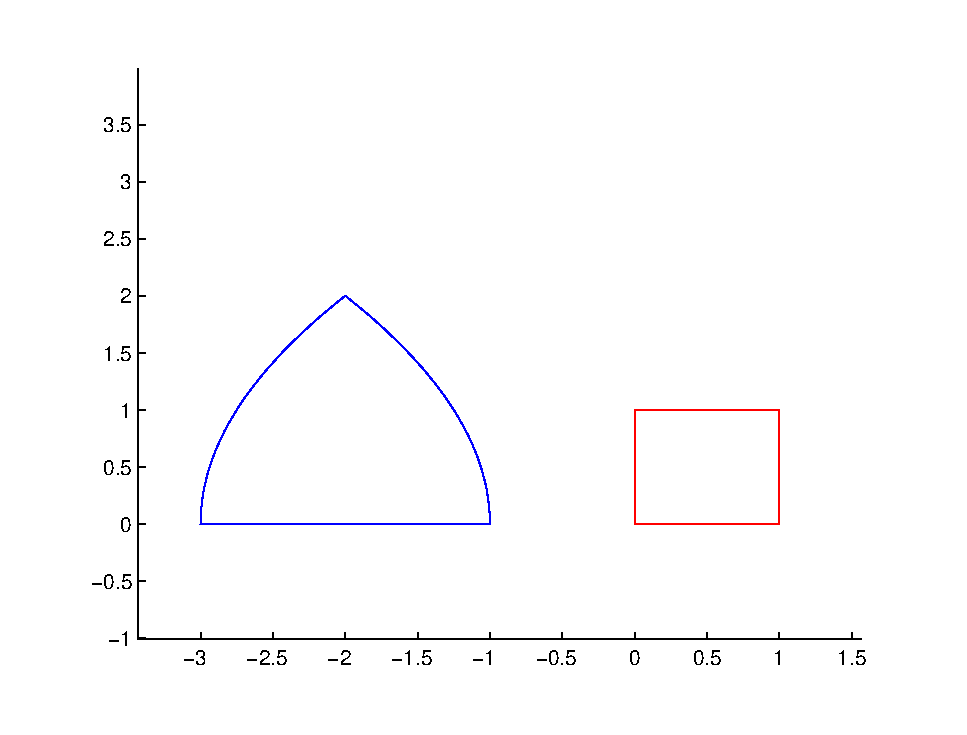
\includegraphics[scale=0.5]{map1}
\caption{The box $[0,1]\times[0,i]$ under g(z).  The vertical axis is the imaginary line and the horizontal axis is the real line.}
\end{center}
\end{figure}

\begin{figure}
\begin{center}
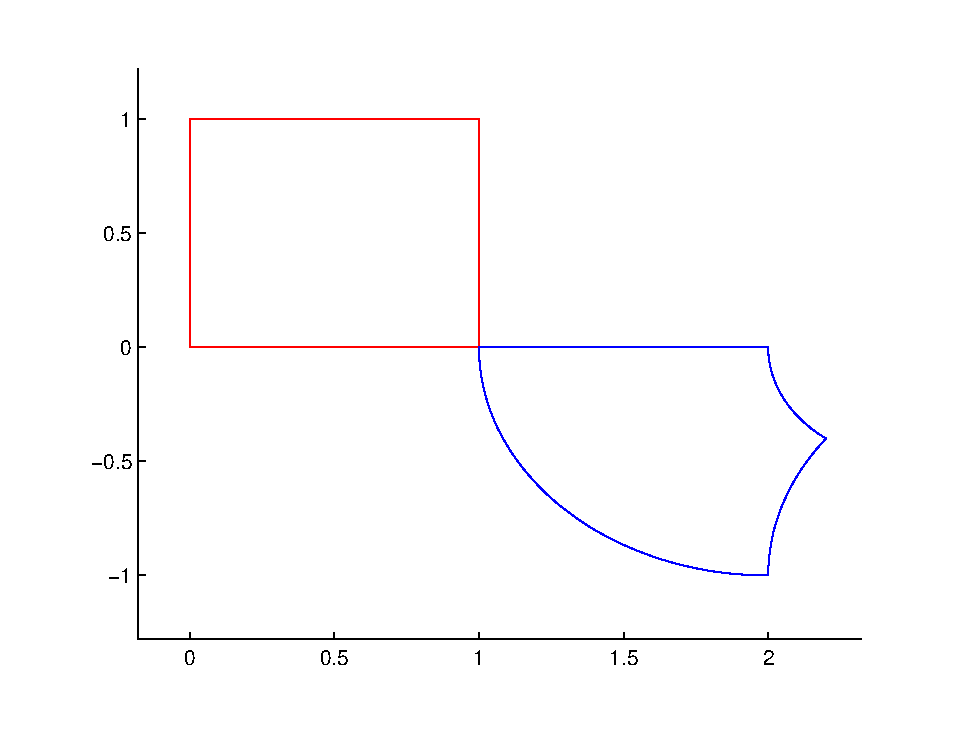
\includegraphics[scale=0.5]{map2}
\caption{bla bla bla}
\end{center}
\end{figure}

There is a fundamental difference between these two mappings.  Though in both cases the shape is significantly distorted, in the case of $f(z)$ the angles where two sides meet are preserved, whereas $g(z)$ distorts not only the shape of the lines but also the angles where they meet.  Maps that preserve angles, as in the case of $f(z)$, are called conformal.

\begin{figure}
\begin{center}
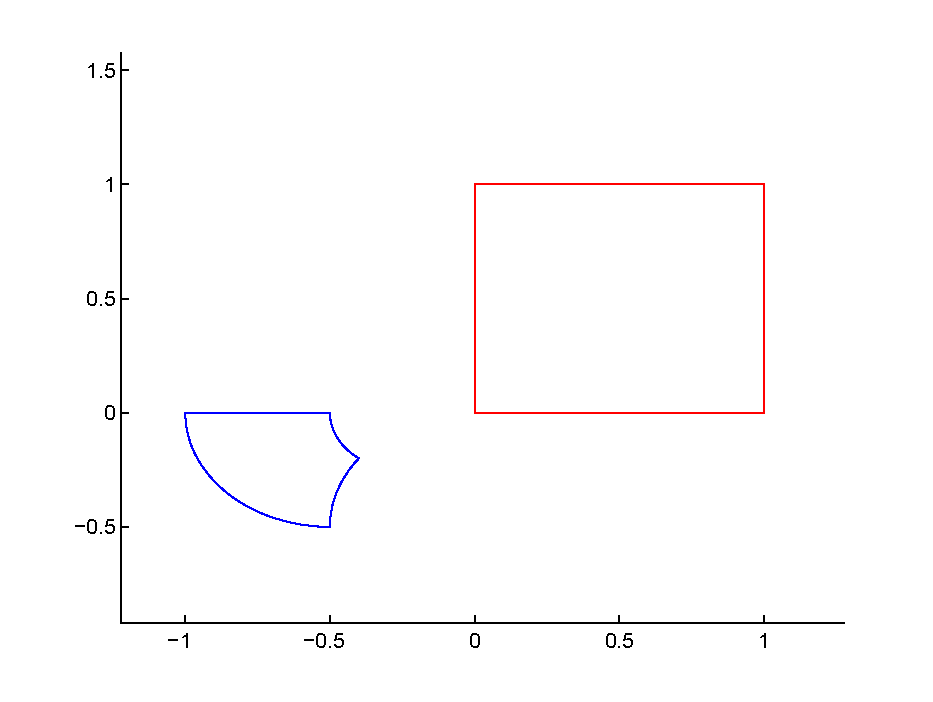
\includegraphics[scale=0.33]{map3}
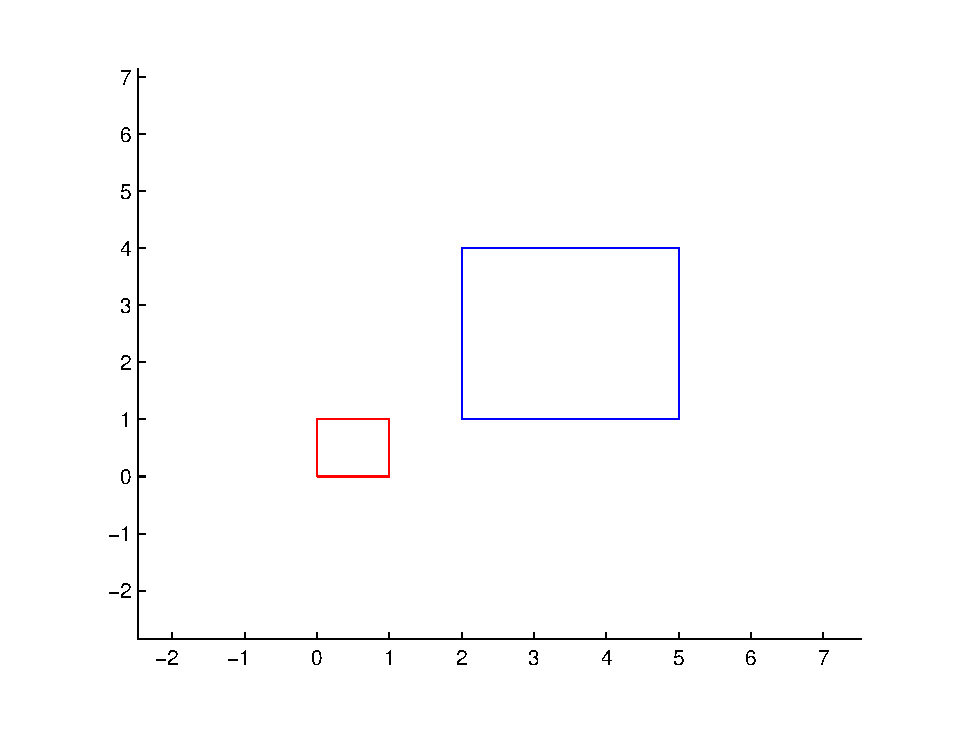
\includegraphics[scale=0.33]{map4}
%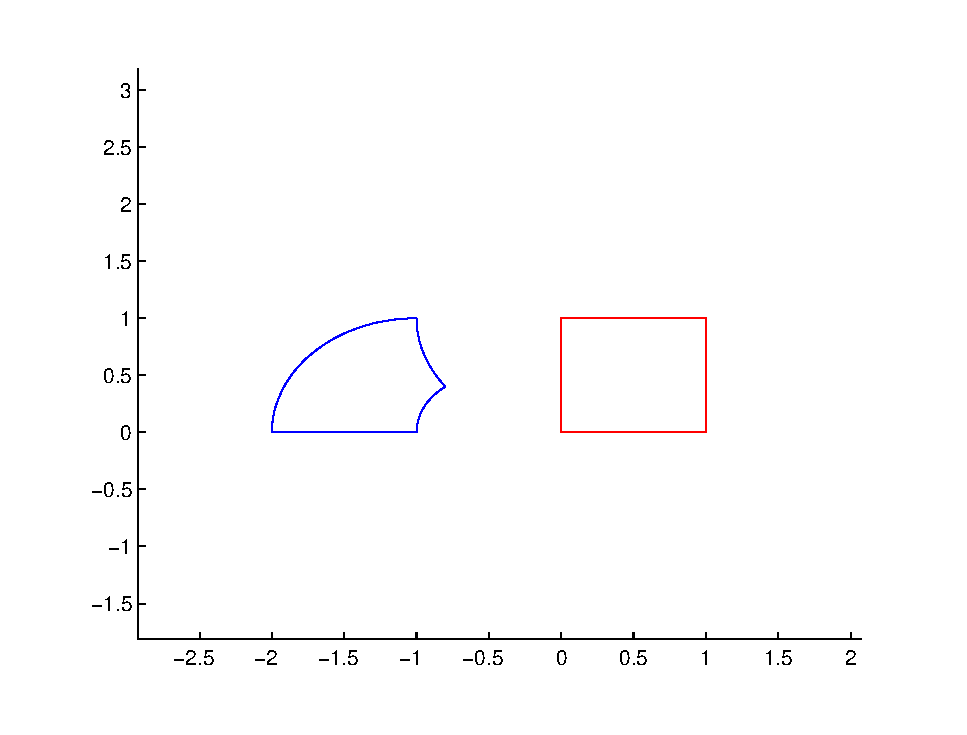
\includegraphics[scale=0.33]{./Applications_Labs/ConfMaps/map5}
\caption{Some more conformal maps}
\end{center}
\end{figure}

\begin{problem}
Write a \ProgrammingLanguage script that transform a shape on the complex plane using the the conformal maps that we have used in the examples.  What do you expect will happen to the unit circle on the complex plane under these transformations?  Do your predictions match the results?  Try this for several shapes.
\end{problem}

The theory of conformal mappings is highly developed and well studied.  Here we only scratch the surface and comment on an important theorem for applications that will be useful in later volumes.

\section*{The Schwarz-Christoffel Transformation}
This transformation is very useful in applications of complex analysis.  Once again, the theory behind this is very rich, and we only state a theorem and look at some simple implications here.

\begin{theorem}  Let $P$ be a polygon on the complex plane having consecutive corners at $z_1, z_2, ..., z_n$ with corresponding right turn angles $\theta_1, \theta_2,...\theta_n$.  Then there exists a function that is a one to one conformal map from the upper half plane onto the interior of $P$ of the form:
\[
f(z) = A\int_0^z (\zeta - x_1)^{\frac{\theta_1}{\pi}}..(\zeta - x_{n-1})^{\frac{\theta_{n-1}}{\pi}}d\zeta + B
\]
Where $\theta_i$ represents the angle made by adjacent sides of the polygon and $x_i \in \mathbb{R}$.
\end{theorem}

We omit the proof here.  Consider the power of this theorem - we are able to map the upper half of the complex plane onto a polygon of our choosing.  This is very powerful for finding the numerical solutions to differential equations that model physical systems.  It turns out that a conformal mapping retains sufficient structure of a domain so that a solution in a transformed domain will be the same as the solution in the original domain.  This fact along with the theorem allows us to take problems which may be very difficult to solve in one domain and transform the domain to a polygonal domain of our choosing where a solution is much easier to find.  We give an example of such a transformation using built in \ProgrammingLanguage functions:

\begin{example}
We will give an example showing how to find a Schwarz-Christoffel transform.  Suppose we wish to transform the upper half plane onto the triangle with corners at $0, i,$ and $1$.  We choose $x_1 = -1$ and $x_2 = 1$.  Starting from the upper corner, we have $\theta_1 = \theta_2 = \frac{-3\pi}{4}$ and $\theta_3 = \frac{-\pi}{2}$.  Using theorem 36.1, we have an expression for our mapping:
\begin{align*}
f(z) &= A\int_0^z(\zeta + 1)^{\frac{-3}{4}}(\zeta - 1)^{\frac{-3}{4}}d\zeta + B \\
	 &= A\int_0^z(\zeta^2 - 1)^{\frac{-3}{4}}d\zeta + B
\end{align*}

\end{example}

\begin{problem}
Find the conformal map that transforms the upper half plane to the strip $|Re(z) < 1|, Im(z) > 0$.  Display the result in a meaningful way.
\end{problem}
